
 Domaines d’application de l’IIoT







\section{Automates Existants et Ajout du Bloc de Communication}
The laboratory's existing Siemens S7-300 PLCs are well-known for their dependability and technical excellence. These controllers, which have been in place since the late 1990s and early 2000s, continue to utilize the same codes today. Although they are well-suited to a range of control and automation activities, their restricted connection posed a significant issue, with the MPI port being the only accessible choice.




\subsection{Caractéristiques principales du S7-300 :}
\begin{itemize}
    \item Input/output modules are adaptable and extensible to meet unique laboratory requirements.
    \item Processor (CPU): A high-performance device capable of processing complicated tasks in real time.
    \item Communication Interfaces: Initially restricted, but require updating to increase connectivity.
\end{itemize}
\subsection{Ajout du Bloc de Communication CP343-1 Lean:}
In order to overcome the S7-300's connectivity constraints, we implemented the CP343-1 Lean communication module. This block has Ethernet connectivity, making it simple to join PLCs with other systems.
The CP 343-1 Lean offers quick, reliable data interchange across several industrial devices, which is an important part of this automation project.

\subsection{Caractéristiques principales du CP343-1 Lean :}

\begin{itemize} 
\item \textbf{Interface Ethernet :} Allows for rapid and reliable connectivity with local area networks (LANs). Supports common protocols including TCP/IP, ISO-on-TCP, and UDP.

\item \textbf{Compatibilité :} Easily integrates with SIMATIC S7-300 PLCs. Simplifies adoption inside existing systems.
\item \textbf{Performance :}
\begin{itemize} 
\item Supports up to 12 simultaneous connections, which fulfills the demands of industrial multitasking situations.
\item Ensures quick transmission, with reaction times ranging from 2.5 to 5 ms, making it excellent for mission important applications.

\end{itemize} 
\item \textbf{Sécurité et Diagnostic :} Fixed MAC address for unique identification on the network.
Includes status LEDs for easy diagnosis of operation and communication.
\item \textbf{Configuration :} Supports flexible configuration via STEP 7 and allows dynamic or manual IP addressing based on network constraints.
\begin{figure}[H]
    \centering
    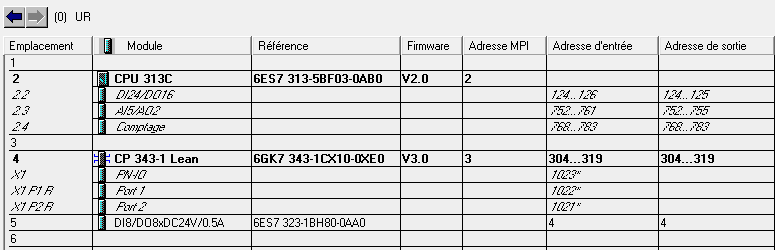
\includegraphics[width=1\textwidth]{chapters/5/img/cp343.png}
    \caption{cp 242-1 LEAN}
    \label{fig:campus}
\end{figure}


\end{itemize}